\documentclass{article}


\usepackage{amsmath} % math stuff
\usepackage{amssymb} % math stuff
\usepackage{array} % equations and stuff
\usepackage{bm} % bold math
%\usepackage{caption} % suppressed table numbering; incompatible with revtex, and longtable, I think
\usepackage{comment} % comment environment
%\usepackage{enumitem} % customization of enumeration, itemize, and description
\usepackage[T1]{fontenc} % font encoding for special characters, must also use scalable font package
\usepackage[margin=0.8in]{geometry} % paper sizes and margins (but be careful not to mess up pre-defined pages)
\usepackage{graphicx} % for graphics
%\usepackage{helvet} % default font is the helvetica postscript font
\usepackage{lipsum} % lorem ipsum filler text
\usepackage{lmodern} % scalable font?
\usepackage{longtable} % multi-page tables
\usepackage{mathrsfs} % math script font
\usepackage{mhchem} % easier chemical formula
\usepackage{microtype} % allows disabling of ligatures
%\usepackage{newcent} % new century schoolbook font
\usepackage{nicefrac}
\usepackage{parskip} % removes paragraph indentation, and adjusts paragraph skip, as well as list items
%\usepackage{setspace} % adjust text spacing and indents
\usepackage{siunitx} % decimal alignment
\usepackage{subfigure} % divided figures
%\usepackage{tabu} % extra table options
\usepackage{textcomp} % symbols
\usepackage{threeparttablex} % better footnotes with longtable
\usepackage{titling} % title placement
%\usepackage{url} % superceded by hyperref
\usepackage{verbatim} % verbatim environment
\usepackage{xcolor} % colors and color boxes
\usepackage{xspace} % commands that don't eat up white space
\usepackage{hyperref} % links and page setup; should always come last

\hypersetup{
	bookmarks=true,
	colorlinks=true,
	citecolor=blue,
	linkcolor=blue,
	urlcolor=blue,
	pdfstartview={XYZ null null 1.0} % default open view is 100%
}

\DisableLigatures[f]{encoding = *, family = * } % disable ff, fi, fl ligatures, without f option, it also disables -- = endash

% allow for vertical lines in bracketed matrix?
\makeatletter
\renewcommand*\env@matrix[1][*\c@MaxMatrixCols c]{%
  \hskip -\arraycolsep
  \let\@ifnextchar\new@ifnextchar
  \array{#1}}
\makeatother

\renewcommand*{\arraystretch}{1.5} % extra vertical space in matrix

\begin{document}

\pagestyle{empty} % don't number pages

%\maketitle

% custom title
\begin{center}
{\LARGE Classic Riddler}

\vspace{0.15in}

{\Large 17 January 2020}
\end{center}


\section*{Riddle:}

After a long night of frivolous quackery, two delirious ducks are having a difficult time finding each other in their pond.
The pond happens to contain a $3\times3$ grid of rocks.

Every minute, each duck randomly swims, independently of the other duck, from one rock to a neighboring rock in the $3\times3$ grid — up, down, left or right, but \textit{not} diagonally.
So if a duck is at the middle rock, it will next swim to one of the four side rocks with probability 1/4.
From a side rock, it will swim to one of the two adjacent corner rocks or back to the middle rock, each with probability 1/3.
And from a corner rock, it will swim to one of the two adjacent side rocks with probability 1/2.

If the ducks both start at the middle rock, then on average, how long will it take until they’re at the same rock again?
(Of course, there’s a 1/4 chance that they’ll swim in the same direction after the first minute, in which case it would only take one minute for them to be at the same rock again.
But it could take much longer, if they happen to keep missing each other.)

\textit{Extra credit}: What if there are three or more ducks? If they all start in the middle rock, on average, how long will it take until they are all at the same rock again?


\section*{Solution:}

At the most basic (and naive) level, there are $9^{2}=81$ possible positions of the ducks, of which nine correspond to the ducks in the same position.
Trying to do this math sounds like a lot of work.
But this can be greatly simplified by noticing that several of the positions are just rotated versions of other positions.
For non-matching positions there are exactly five distinct positions, shown and labeled below:

\vspace{0.2in}
\begin{center}
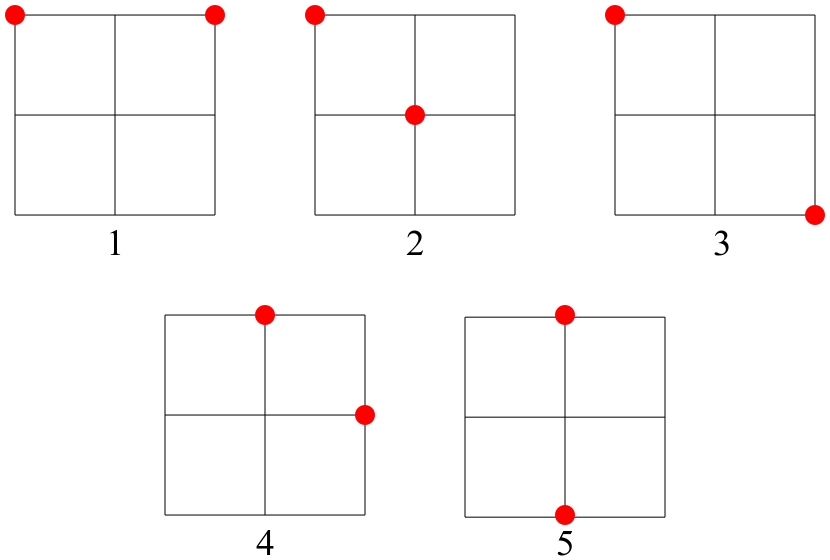
\includegraphics[width=5in]{all_scenarios.png}
\end{center}
\vspace{0.2in}

With just a bit of thinking about these positions, it is relatively easy to deduce what the probabilities are to move between each position or go to a matching position.
I will label all matching positions as position 0.
From position 1, there is a \nicefrac{1}{2} chance to move to 4, a \nicefrac{1}{4} chance to move to 5, and \nicefrac{1}{4} chance to match.
Position 2 has identical probabilities.
From position 3, there is a \nicefrac{1}{2} chance to move to 4 and a \nicefrac{1}{2} chance to move to 5.
From position 4, there is a \nicefrac{2}{9} chance to move to 1, a \nicefrac{4}{9} chance to move to 2, a \nicefrac{1}{9} chance to move to 3, and \nicefrac{2}{9} to match.
From position 5, there is a \nicefrac{2}{9} chance to move to 1, a \nicefrac{4}{9} chance to move to 2, a \nicefrac{2}{9} chance to move to 3, and \nicefrac{1}{9} to match.
So now that I have the numbers sorted out, how do I solve the riddle?

My first instinct was to set up a simulation, with a position variable that changes from 0--5, and a counter that keeps track of the number of moves to get to a match.
Then I would just run the simulation a few million times and take the average number of moves.
But I realized I could set up a system of equations.
I just need to relate the average number of moves from any position to the average numbers of moves from the other positions.
Letting $N_{i}$ be the average number of moves from position $i$, I set up the equations as follows:

\[
N_{0}=0
\]
\[
N_{1}=\frac{1}{4}(1+N_{0})+\frac{1}{2}(1+N_{4})+\frac{1}{4}(1+N_{5})
\]
\[
N_{2}=\frac{1}{4}(1+N_{0})+\frac{1}{2}(1+N_{4})+\frac{1}{4}(1+N_{5})
\]
\[
N_{3}=\frac{1}{2}(1+N_{4})+\frac{1}{2}(1+N_{5})
\]
\[
N_{4}=\frac{2}{9}(1+N_{0})+\frac{2}{9}(1+N_{1})+\frac{4}{9}(1+N_{2})+\frac{1}{9}(1+N_{3})
\]
\[
N_{5}=\frac{1}{9}(1+N_{0})+\frac{2}{9}(1+N_{1})+\frac{4}{9}(1+N_{2})+\frac{2}{9}(1+N_{3})
\]

Each term has a 1 because it takes exactly 1 move to get to the new position from the old position.
So now I just have to solve these equations.
Rearranging them (and removing the trivial $N_{0}$ terms) gives the following system:

\[
N_{1}-\frac{1}{2}N_{4}-\frac{1}{4}N_{5}=1
\]
\[
N_{2}-\frac{1}{2}N_{4}-\frac{1}{4}N_{5}=1
\]
\[
N_{3}-\frac{1}{2}N_{4}-\frac{1}{2}N_{5}=1
\]
\[
-\frac{2}{9}N_{1}-\frac{4}{9}N_{2}-\frac{1}{9}N_{3}+N_{4}=1
\]
\[
-\frac{2}{9}N_{1}-\frac{4}{9}N_{2}-\frac{2}{9}N_{3}+N_{5}=1
\]

The easiest way to solve this is to plug in a matrix into Wolfram Alpha and have it row-reduce the matrix.
The matrix becomes

\[
\begin{bmatrix}[ccccc|c]
1            & 0            & 0            & -\frac{1}{2} & -\frac{1}{4} & 1 \\
0            & 1            & 0            & -\frac{1}{2} & -\frac{1}{4} & 1 \\
0            & 0            & 1            & -\frac{1}{2} & -\frac{1}{2} & 1 \\
-\frac{2}{9} & -\frac{4}{9} & -\frac{1}{9} & 1            & 0            & 1 \\
-\frac{2}{9} & -\frac{4}{9} & -\frac{2}{9} & 0            & 1            & 1
\end{bmatrix}
\]
with solution

\[
\begin{bmatrix}[ccccc|c]
1 & 0 & 0 & 0 & 0 & \frac{363}{74} \\
0 & 1 & 0 & 0 & 0 & \frac{363}{74} \\
0 & 0 & 1 & 0 & 0 & \frac{234}{37} \\
0 & 0 & 0 & 1 & 0 & \frac{184}{37} \\
0 & 0 & 0 & 0 & 1 & \frac{210}{37}
\end{bmatrix}
\]

One final observation is that the probability distribution with both ducks moving away from the center rock is the same distribution as from position 2.
So I can take the value of $N_{2}$, and the solution is
\fcolorbox{red}{white}{$\frac{363}{74}\approx4.905$}\,.

Solving the extra credit would mean setting up a more complex set of positions for different numbers of ducks, identifying the probabilities of moving between them, and inputting the equations into Wolfram Alpha.
This is probably easy enough for three ducks, and at least do-able for four ducks.
But it would take more time than I'm willing to put in.


\end{document}